\chapter{Hierarchical Temporal Memory(HTM)}
\section{HTMの概要}
HTMは大脳皮質の構造と学習アルゴリズムを模して作られたニューラルネットワークである。
構造はカラムとセルによる2次元マップ表現となっており、各セルが状態を偏移させる。
学習アルゴリズムはヘブ則となっており各時刻間で活性化状態のセル同士の接続を強める。
また活性化状態のセルと強く接続しているセルが予測状態に遷移することで予測を行う。

HTMの特徴は疎な分散表現を用いたことによる並列同時予測が可能な点とネットワークの欠損に強いという点がある。

\section{HTMの構造}
HTMの全体構造を下の図1に示す。

\begin{center}
  \begin{figure}[ht]
    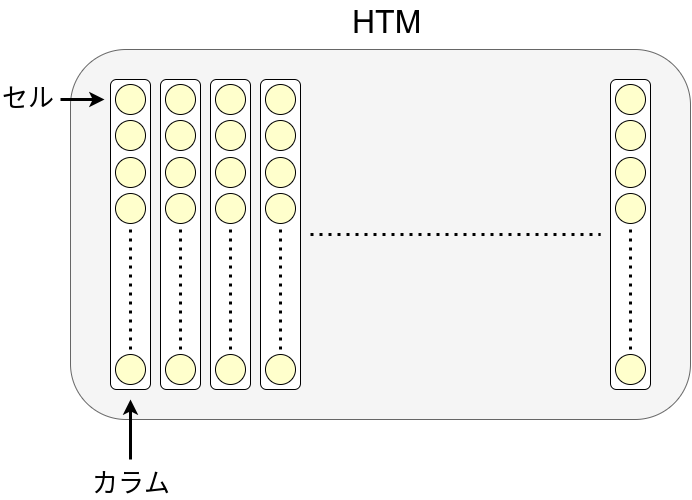
\includegraphics[scale=0.5]{./fig/drawing_1}
    \caption{HTMの全体構造}
    \label{fig:HTM}
  \end{figure}
\end{center}

\subsection{セルの状態変化}
\subsection{パターン表現}
\subsection{セル内の構造}
\subsection{疎な分散表現}


\section{HTMの学習アルゴリズム}
\subsection{活性化状態の計算}
\subsection{予測状態の計算}
\subsection{セグメント集合を用いた接続値の更新}


\section{HTMの問題点}
\begin{itemize}
  \item 疎な分散表現を用いたために発火するセルが徐々に少なくなり消失する。
  \item 学習が大きく進んだパターンにおいて表現が疎になった時に次のパターンに繋がっていたセルが消失するために学習が損失
\end{itemize}
